\section[化学键]{化学键} \label{sec:10.05} % 
% \makebox[5em][s]{} % 短题目拉间距

分子或晶体中将原子结合在一起的力都来自带电粒子间的库仑作用力.(和自旋有关的作用如自旋轨道耦合作用是微不足道的)按照键的物理机制和表现形式,大致分为离子键,共价键,金属键等类型.

正、负离子由于库仑吸引力而结合,就形成离子键.这种键的性质大体上用经典物理(静电学)就可以解释.如$\ce{Na^{+}}\ce{Cl^{-}}$晶体就是典型离子键晶体.

在共价键分子(或晶体)中,由于电子波函数的交换对称性,价电子比较集中地出现在二原子之间,通过它们与原子(离子)间的库仑吸引力而起键合作用.氢分子就是典型的共价键分子.共价键的形成,电子波函数的交换对称性起关键作用,是典型的量子力学效应,没有经典物理解释.

金属键是能带电子在晶体中公有化,在整个晶体中流动而产生的键合作用,性质接近共价键.金属键的概念来自固体物理,现已逐渐应用于量子化学,用来解释某些有机分子(如苯)的结构.

本节主要讨论共价键.由于篇幅所限,只作初浅的定性介绍.

上节讨论的氢分子是共价键分子的简单实例.两个原子间形成共价键时,通常“交换能”是负的,而且其绝对值远大于“库仑能”,结果导致构成键的一对电子处于自旋单态(反对称态)和轨道对称态,即$\Psi(q_{1},q_{2})=\chi_{00}(S_{1z}S_{2z})\varPsi^{S}(\boldsymbol{r}_{1},\boldsymbol{r}_{2})$,当两个电子位贸接近$(\boldsymbol{r}_{1}\sim\boldsymbol{r}_{2})$并处于两原子之间时,$|{\varPsi^{S}}|^{2}$较大,因此可以认为这一对价电子是被两个原子共同占有,共价键的名称即由此而来.

\begin{wrapfigure}[9]{r}{8em}
	\centering
	\small
	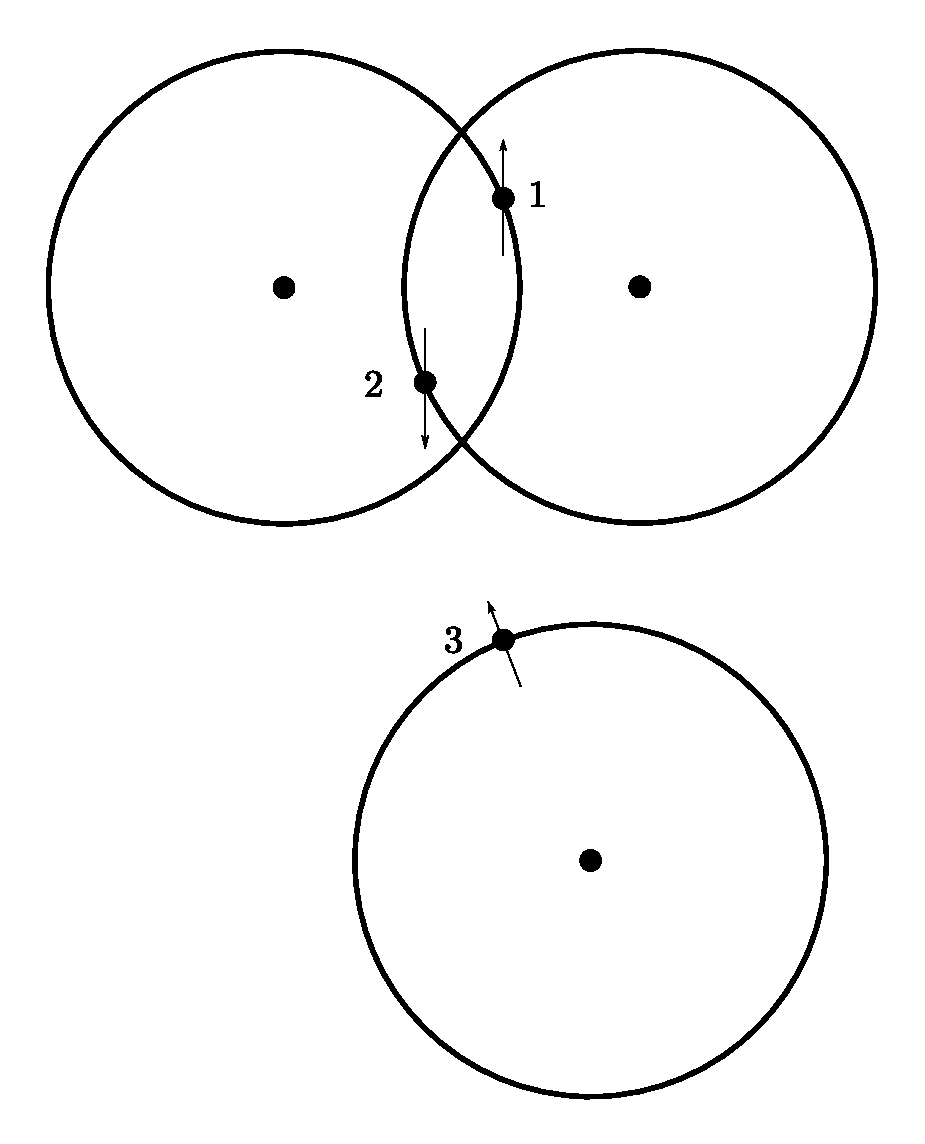
\includegraphics[width=2.5cm,clip]{QM file/figure/10-7}
	\caption{}\label{fig.10-7}
\end{wrapfigure}

共价键最显著的特点是饱和性.设想有第三个氢原子接近一个氢分子.后者的电子对已经处于自旋反对称态,两电子的自旋指向相反,总自旋为0.
外来的第三个电子已经不可能再与它们构成自旋反对称态,所以不能再形成键.从概率观点看问题,两个自旋指向混乱的电子(外来原子的电子与分子中的一个电子,参看图\ref{fig.10-7}),构成自旋对称态(三重态$\chi_{11},\chi_{10},\chi_{1-1}$)的概率是$\frac{3}{4}$,构成自旋反对称态(单态,$\chi_{00}$)的概率是$\frac{1}{4}$,而自旋对称态必为轨道反对称态,原子间的作用$(V^{A})$是排斥的结果是外来原子将受排斥.这就是共价键的饱和性.离子键就没有这种饱和性.

共价键的另一个特点是有方向性.共价键的形成是两个原子的价电子云重叠$(\boldsymbol{r}_{1}\sim\boldsymbol{r}_{2})$的结果,因此形成键的方向总是在价电子云的极大方向.氢原子中电子处于1s态,电子云分布各向同性,没有方向性,第二个原子可以从任何方向接近第一个原子而形成共价键,这种键没有方向性.如果原子的价电子是p态$(l=1)$或d态$(l=2)$电子,其电子云分布就有方向性.以p电子为例,共有3种独立轨道状态,即
\begin{empheq}{equation}\label{eqx5.1}
	\begin{aligned}
		&\varPsi_{npz}=\varPsi_{n10}=zF(r)	\\
	\varPsi_{npx}&=\frac{1}{\sqrt{2}}(\varPsi_{n1-1}-\varPsi_{n11})=xF(r)	\\
	\varPsi_{npy}&=\frac{i}{\sqrt{2}}(\varPsi_{n1-1}+\varPsi_{n11})=yF(r)
	\end{aligned}
\end{empheq}
电子云密度$\varPsi^{2}$的极大方向分别是$x,y,z$轴方向,如另一个原子的价电子(设为s电子)与这样的p电子构成共价键,键的方向必为p电子云的极大方向,如图\ref{fig.10-8}所示.

\begin{figure}[!h]
	\centering
	\small
	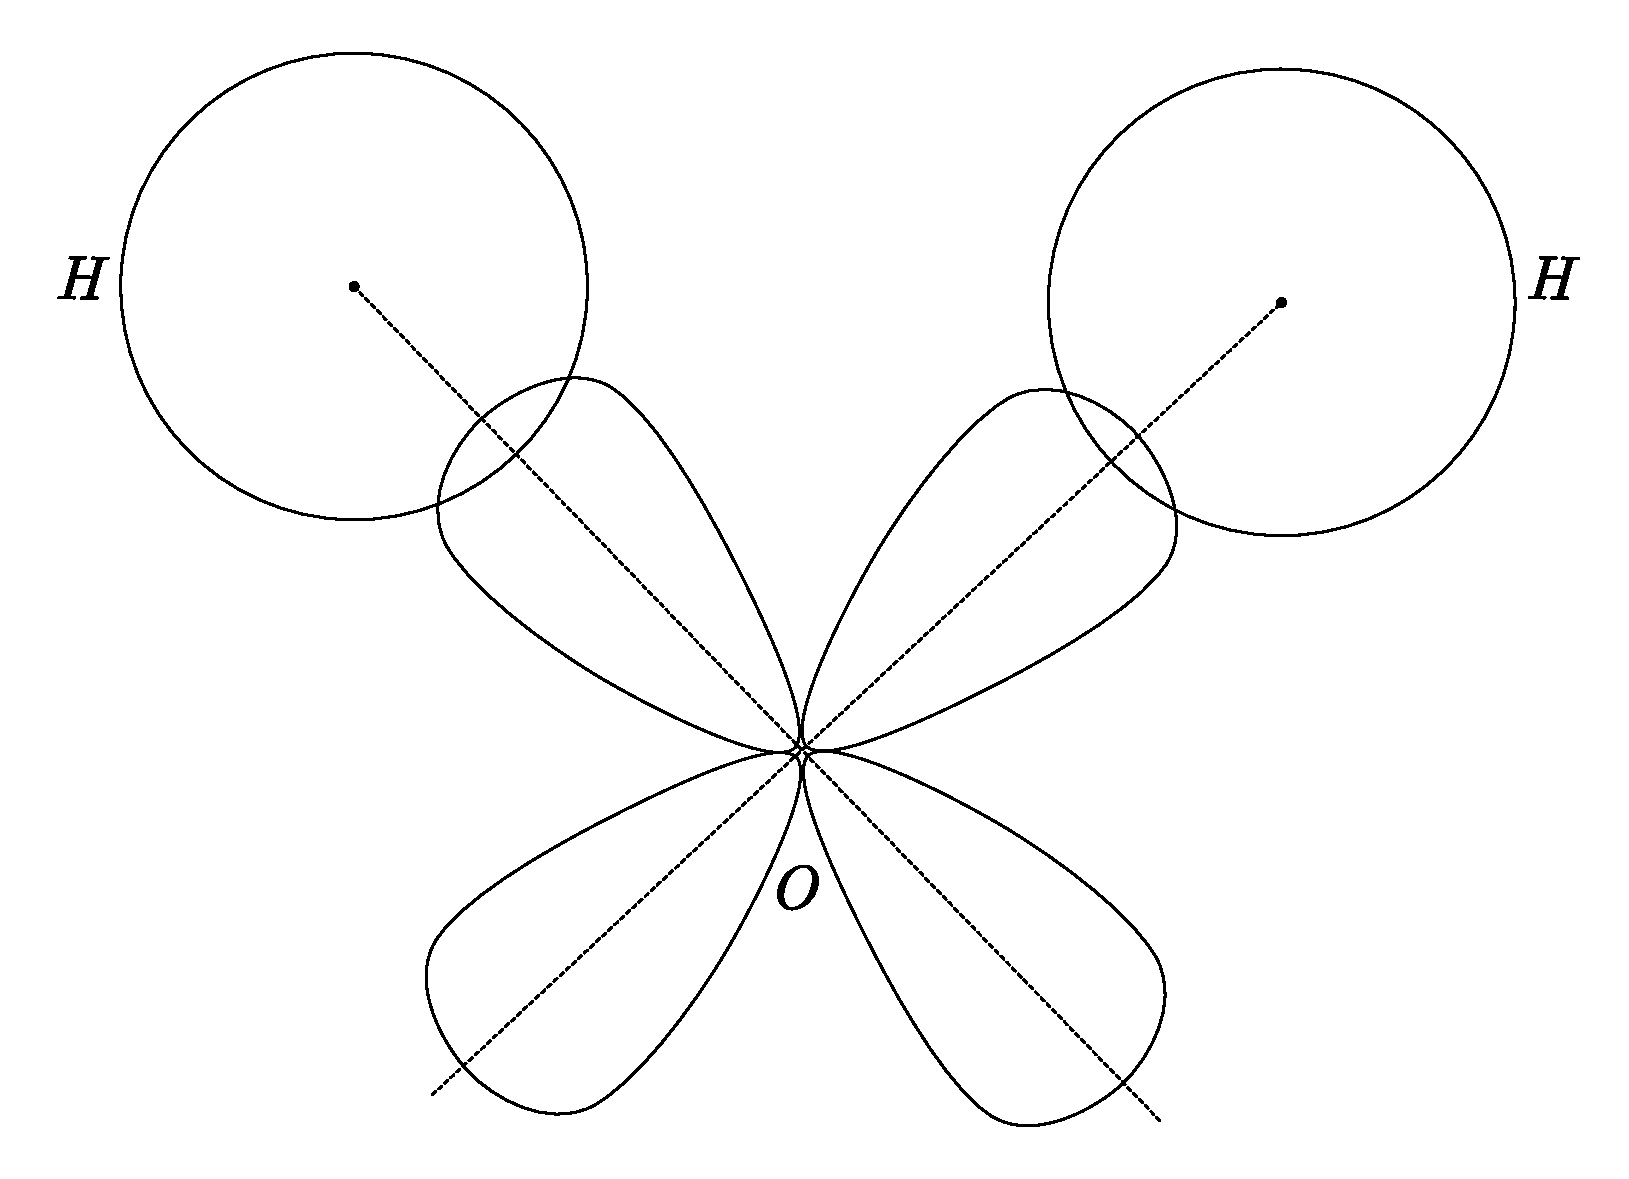
\includegraphics[width=7cm,clip]{QM file/figure/10-8}
	\caption{}\label{fig.10-8}
\end{figure}

以水$\ce{H_{2}O}$分子为例.氧原子中参与$\ce{H-O}$键的两个电子都是p电子,它们电子云的极大方向相互成$90^{\circ}$角.这两个p电子各自和一个氢原子的1s电子结合成共价键,如图\ref{fig.10-8}.由于$\ce{H-O}$键有少量离子键的因素(即$\ce{H^{+}-O^{--}-H^{+}}$),两个氢原子(离子)互相排斥,键角实际上增大成$105^{\circ}$.在19世纪,化学界曾想当然地以为$\ce{H_{2}O}$分子是直线式构造$\ce{H-O-H}$,有了量子化学,键的方向性概念以量子力学为理论依据,才被普遍承认.

在分子中,参与键的电子,由于受到邻近原子的影响,其原子状态严格地说已经与成键前不同.特别是,由于作用势的球对称性(各向同性)遭到破坏,价电子可以不再保持单一的$\boldsymbol{L}^{2}$本征值,其状态可以是s,p,d态的杂化态,这种处于杂化轨道的电子,其电子云分布更容易集中到某个方向,因此更有利于键的形成.量子化学利用杂化轨道理论成功地解释了许多分子构造问题.例如甲烷$(\ce{CH_{4}})$分子,碳$(\ce{C})$原子参与$\ce{C-H}$键的4个电子,本来的原子轨道是$(\ce{2s})^{2}(\ce{2p})^{2}$,由于轨道杂化,它们的单电子轨道态变成如下形式,
\begin{empheq}{equation}\label{eqx5.2}
	\varPsi(\boldsymbol{r})=a\varPsi_{\ce{2s}}+b\varPsi_{\ce{px}}+c\varPsi_{\ce{2py}}+d\varPsi_{\ce{2pz}}
\end{empheq}
当$(a,b,c,d)$取$(1,1,1,1)$,$(1,1,-1,-1)$,$(1,-1,1,-1)$,$(1,-1,-1,1)$时,电子云极大方向刚好是从正四面体中心指向4个顶点的方向,氢原子从这些方向接近,就容易结合成$\ce{C-H}$键.所以$\ce{CH_{4}}$分子中,4个$\ce{H}$原子正好处于正四面体顶点的位置,而$\ce{C}$原子处于对称中心.

半个多世纪以来,由于计算技术的进步和广泛运用量子力学理论及近似方法,量子化学已经发展成一门卓有成效的学科.


